\documentclass[a4paper,
fontsize=11pt,
%headings=small,
oneside,
numbers=noperiodatend,
parskip=half-,
bibliography=totoc,
final
]{scrartcl}

\usepackage{synttree}
\usepackage{graphicx}
\setkeys{Gin}{width=.8\textwidth} %default pics size

\graphicspath{{./plots/}}
\usepackage[ngerman]{babel}
\usepackage[T1]{fontenc}
%\usepackage{amsmath}
\usepackage[utf8x]{inputenc}
\usepackage [hyphens]{url}
\usepackage{booktabs} 
\usepackage[left=2.4cm,right=2.4cm,top=2.3cm,bottom=2cm,includeheadfoot]{geometry}
\usepackage{eurosym}
\usepackage{multirow}
\usepackage[ngerman]{varioref}
\setcapindent{1em}
\renewcommand{\labelitemi}{--}
\usepackage{paralist}
\usepackage{pdfpages}
\usepackage{lscape}
\usepackage{float}
\usepackage{acronym}
\usepackage{eurosym}
\usepackage[babel]{csquotes}
\usepackage{longtable,lscape}
\usepackage{mathpazo}
\usepackage[normalem]{ulem} %emphasize weiterhin kursiv
\usepackage[flushmargin,ragged]{footmisc} % left align footnote

\usepackage{listings}

\urlstyle{same}  % don't use monospace font for urls

\usepackage[fleqn]{amsmath}

%adjust fontsize for part

\usepackage{sectsty}
\partfont{\large}

%Das BibTeX-Zeichen mit \BibTeX setzen:
\def\symbol#1{\char #1\relax}
\def\bsl{{\tt\symbol{'134}}}
\def\BibTeX{{\rm B\kern-.05em{\sc i\kern-.025em b}\kern-.08em
    T\kern-.1667em\lower.7ex\hbox{E}\kern-.125emX}}

\usepackage{fancyhdr}
\fancyhf{}
\pagestyle{fancyplain}
\fancyhead[R]{\thepage}

%meta
%meta

\fancyhead[L]{J. Wonke-Stehle \\ %author
LIBREAS. Library Ideas, 30 (2016). % journal, issue, volume.
\href{http://nbn-resolving.de/
}{}} % urn
\fancyhead[R]{\thepage} %page number
\fancyfoot[L] {\textit{Creative Commons BY 3.0}} %licence
\fancyfoot[R] {\textit{ISSN: 1860-7950}}

\title{\LARGE{Rezension zu: Ulrich Herb (2015). \emph{Open Science in der Soziologie: Eine interdisziplinäre Bestandsaufnahme zur offenen Wissenschaft und eine Untersuchung ihrer Verbreitung in der Soziologie}. Glückstadt: vwh.
}} %title %title
\author{Jens Wonke-Stehle} %author

\setcounter{page}{1}

\usepackage[colorlinks, linkcolor=black,citecolor=black, urlcolor=blue,
breaklinks= true]{hyperref}

\date{}
\begin{document}

\maketitle
\thispagestyle{fancyplain} 

%abstracts

%body
\section*{Kontext}\label{kontext}

Open Science ist ein wissenschaftspolitisches Konstrukt, das derzeit von
vielen Akteuren aufgegriffen wird.

\begin{quote}
\enquote{Der Begriff {[}\ldots{}{]} bündelt Strategien und Verfahren,
die allesamt darauf abzielen, die Chancen der Digitalisierung konsequent
zu nutzen, um alle Bestandteile des wissenschaftlichen Prozesses über
das Internet offen zugänglich und nachnutzbar zu machen.} (Open
Knowledge Foundation 2016)
\end{quote}

Durch die Zusammenführung von mittlerweile etablierten technischen
Möglichkeiten der netzbasierten Zusammenarbeit einerseits und denen der
digitalen Verbreitung von Wissen andererseits sollen so bisherige,
analoge Limitationen des Forschungsprozesses überwunden werden:

\begin{quote}
\enquote{Der offene, durch möglichst wenige finanzielle, technische und
rechtliche Hürden behinderte Zugang zu wissenschaftlichen Publikationen,
Forschungsdaten und wissenschaftlicher Software erweitert die
Transparenz und die Möglichkeiten zur Qualitätssicherung
wissenschaftlicher Arbeit, erhöht durch eine verbesserte
Informationsversorgung die Leistungsfähigkeit der Wissenschaft und
steigert durch die Erleichterung des Wissenstransfers in Wirtschaft und
Gesellschaft die auf wissenschaftlichen Erkenntnissen basierende
Innovation.} (Helmholtz Gemeinschaft 2016)
\end{quote}

Damit wird die Diskussion um Open Access von der Beschränkung auf den
Publikationsmodus von Texten befreit und die Weiterentwicklung des
gesamten Forschungszyklus in den Blick genommen.

Je nach Perspektive umfasst das Open Science-Bündel neben den bereits
genannten Elementen Publikationen, Forschungsdaten und Software auch
Linked Open Data, Open Review, Citizen Science sowie Open Education und
mündet in einen umfassenden Diskurs zur sogenannten Openness. (vgl. Max
Planck Digital Library 2016)

In welchem Maß sich die Open Science jenseits dieser Postulate bereits
gegenwärtig in der Wissenschaftspraxis manifestiert, untersucht Ulrich
Herb in seiner Dissertation \enquote{Open Science in der Soziologie},
die er hybrid veröffentlicht hat: Digital unter der Creative
Commons-Lizenz CC-BY-NC auf dem Online-Speicherdienst Zenodo sowie auf
dem institutionellen Repositorium SciDok, inklusive Forschungsdaten als
Supplement und schließlich gedruckt im Werner Hülsbusch
Verlag.\footnote{DOI: \url{https://doi.org/10.5281/zenodo.31234} oder
  URN: \url{http://nbn-resolving.de/urn:nbn:de:bsz:291-scidok-62565}}

\section*{Aufbau}\label{aufbau}

Herb geht analog zum Titel in drei Schritten vor: Zuerst leitet er eine
Definition von Offenheit ab (A), trägt anschließend zusammen, was in
dieser Perspektive bereits fachübergreifend praktiziert wird (B) und
fokussiert schließlich auf die Situation in der deutschsprachigen
Soziologie (C).

In Teil A wird das begriffliche Instrumentarium angelegt. Basierend auf
der \enquote{logische{[}n{]} Unterscheidung von entgeltfreiem und
offenem Zugang zu wissenschaftlichen Informationen} (Herb 2015, S. 12)
definiert Herb fünf Untersuchungsdimensionen, die für ihn die
\enquote{Bausteine der}\emph{Offenen Wissenschaft\enquote{* ausmachen:
1. \emph{\enquote{Open Access zu wissenschaftlichen Publikationen},}
2.}}Open Access zu Forschungsdaten``*, 3. ``*Open Review``*, 4.
\enquote{\emph{Open Metrics}} und schließlich 5. ``*Open Access zu
wissenschaftlicher Software.``* (ebd.)

Zusammengenommen ist Open Science damit ein \enquote{Prinzip
{[}\ldots{}{]}, das alle im Forschungszyklus anfallenden
Informationsitems offen oder zumindest entgeltfrei verfügbar machen
will} (ebd. , S. 9).

Ein Zwischenfazit fasst diesen Teil zusammen.

In Teil B referiert Herb fachübergreifend Studien, die
Publikationspraktiken in den fünf Bausteinen der offenen Wissenschaft
empirisch analysiert haben und kommt so zu einer \enquote{Darstellung
des aktuellen Standes der einzelnen Open-Science-Teilbereiche (inklusive
vorgetragener Argumente zugunsten der Konzepte sowie dagegen).} (ebd.,
S. 7) Dieser Teil bildet die Folie, vor der die Situation der Soziologie
beurteilt werden kann. In dieser umfangreichen Metastudie werden in
jeder Dimension im Detail die Begrifflichkeiten und die zentralen
Argumentationsfelder erläutert sowie der jeweilige Stand der Forschung
referiert.

Der dritte Teil (C) ist der Analyse des aktuellen Stands der offenen
Wissenschaft in der deutschsprachigen Soziologie gewidmet. Herb geht es
in diesem Teil um \enquote{eine Untersuchung der Verbreitung und
Akzeptanz der erwähnten fünf Open-Science-Bausteine in der Soziologie
(insbesondere der deutschsprachigen) anhand einer Literaturstudie und
explorativer Datenerhebungen.} (ebd., S. 8) Die Ergebnisse seiner
eigenen Erhebungen sind, soweit es die rechtlichen Bedingungen
erlaubten, als Supplement zum Dissertationstext veröffentlicht. (vgl.
z.B. Herb 2014)

Für seine eigenen Erhebungen in diesem Abschnitt stellt Herb basierend
auf den Erkenntnissen der ersten beiden Teile vier Hypothesen auf:

\begin{enumerate}
\def\labelenumi{\Alph{enumi}.}
\item
  \enquote{Open Access zu wissenschaftlichen Journalen und
  Journalartikeln ist in der Soziologie nicht geringer ausgeprägt als in
  anderen Disziplinen.} (Herb 2015, S. 321)
\item
  \enquote{Open Access zu wissenschaftlichen Buchpublikationen ist in
  der Soziologie geringer ausgeprägt als der Open Access zu Journalen
  und Journalartikeln.} (ebd.)
\item
  \enquote{Die Open-Science-Elemente offener Zugang zu Forschungsdaten
  und -software, Open Metrics und Open Review finden wenig Verbreitung
  und Anerkennung in der Soziologie.} (ebd., S. 322)
\item
  \enquote{Die metrische Beschreibung von Textpublikation aus der
  Soziologie gelingt durch Zitationsdatenbanken schlechter als durch die
  Nutzung von Altmetrics, Open Metrics oder Google Scholar.} (ebd.)
\end{enumerate}

Herb bricht diese vier Komplexe auf 22 Forschungsfragen herunter, z.B:
\enquote{3. Wenden Open-Access-Journale in den Sozialwissenschaften in
geringerem Maß Peer Review an als Open-Access-Journale aus anderen
Disziplinen? {[}Hypothese A{]}} (ebd.), oder \enquote{15. In welchem
Ausmaß machen Autoren Forschungsdaten zu Artikeln in soziologischen
Journalen frei oder offen zugänglich? {[}Hypothese C{]}} (ebd., S. 323).

Die Studie endet mit einer knappen abschließenden Bewertung.

\section*{Kritik}\label{kritik}

Hier soll kein Peer Review durchgeführt werden, sondern ein Nebeneffekt
der Dissertation überprüft werden, nämlich die Frage, ob es sich lohnt,
sie zu lesen. Und da absolute Aussagen immer schwierig sind, soll diese
Perspektive eingeschränkt werden auf Menschen, die sich in Bibliotheken
berufsmäßig mit in den Geistes- und Sozialwissenschaften Forschenden
beschäftigen, z.B. FachreferentInnen.

Ja. (Und deswegen gibt es hier auch keine Spoiler.)

Herbs Text ist in seiner Anlage älter als die derzeitige Konjunktur des
Begriffs Open Science. Vielleicht ermöglicht gerade das einen so klaren
und wenig dem Hype geschuldeten Zugang: Was bedeutet offen und wie
äußert sich das in Forschungspraktiken? Die beiden ersten Teile sind
dabei so übergreifend und abstrakt angelegt, dass sie für LeserInnen
auch unabhängig von deren Interesse für Soziologie funktionieren. Der
Überblick über Studien zur Verbreitung von Open Science und den Effekten
des offenen Publizierens ist ein äußerst wichtiger Teil der Debatte um
Open Science, weil er mit dem referierten Material den Bezugspunkt für
eine empirisch begründete Auseinandersetzung schafft. Die Fokussierung
auf die Soziologie am Ende ist interessant, weil die Soziologie in der
öffentlichen Wahrnehmung gerade nicht als Paradefach der Open
Access-Kultur gilt. (vgl. Herb 2015, S. 10)

Der Aufbau ist logisch. Es stört lediglich etwas, dass die detaillierte
Fragestellung erst im dritten Teil und damit sehr nah am Schluss nach
zwei Dritteln Text erläutert wird (ohne dass ein Gegenvorschlag nahe
läge, denn was man speziell an der Soziologie untersuchen könnte ergibt
sich nach und nach aus den Begriffsklärungen (A) und dem
fachübergreifenden Überblick (C) ). Die Prüfung der vier Hypothesen
daraufhin, ob sie \enquote{bestätigt} werden können, erscheint
verzichtbar. Sie haben eher den Charakter von empirisch fundierten
Thesen. Die Forschungsfragen sind aber sowohl für die
Bibliothekswissenschaft als auch für die bibliothekarische Praxis
relevant.

Um einen in sich abgeschlossenen Text zu schaffen, der alle Elemente zur
Bearbeitung seiner Forschungsfragen selbst enthält, also gewissermaßen
einen Hypertext, den man offline lesen kann, musste Herb zwangsläufig
eine Vielzahl von Ergebnissen referieren. Er tut das abwechslungsreich,
mal zitiert er indirekt, mal referiert er im Fließtext, mal, wenn es die
Lizenz erlaubt, bettet er Grafiken im Layout der jeweiligen Studie ein
und macht so en passant klar, was \enquote{re-use} bedeutet. Aber dieses
Ansammeln von Input für die Auswertung nimmt viel Raum ein und macht den
Text auch sperrig. So wäre ebenso am Ende von Teil B, dem Überblick über
den Stand der Open Science, ein Zwischenfazit hilfreich gewesen.

Das Werk ist eine große Hilfe für alle, die in Bibliotheken im sozial-
und geisteswissenschaftlichen Umfeld einen Überblick über sich
verändernde Forschungs- und Publikationspraktiken benötigen, da ihnen
eine klare Erläuterung der Terminologie, ein knapper Einstieg in die
Diskussion und ein tiefer Einblick in die aktuelle Wissenschaftspraxis
gegeben wird.

\begin{figure}
\centering
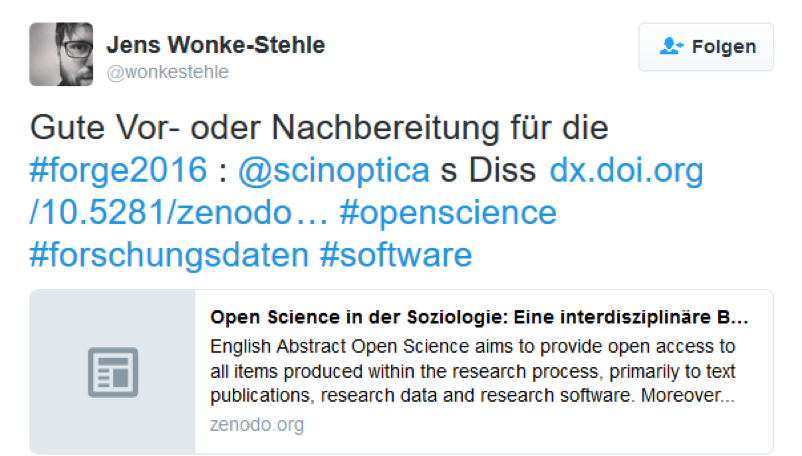
\includegraphics{img/abbildung.png}
\caption{Quelle:
\url{https://twitter.com/wonkestehle/status/776371238210002944}}
\end{figure}

\section*{Literatur}\label{literatur}

Helmholtz Gemeinschaft (2016): Open Science.
\url{https://www.helmholtz.de/forschung/open_science/}.

Open Knowledge Foundation (2016): Open Science.
\url{https://okfn.de/themen/offene-wissenschaft/}.

Max Planck Digital Library: Open Science Days:
About.\url{http://osd.mpdl.mpg.de/}.

Herb, Ulrich (2014): Open Science in Soziologie-Journalen aus
deutschsprachigen und nicht-deutschsprachigen Ländern, Daten und
Auswertungen einer Journal-Stichprobe {[}Data set{]}. Zenodo.
\url{http://doi.org/10.5281/zenodo.10786}.

Herb, Ulrich (2015):~Open Science in der Soziologie:~Eine
interdisziplinäre Bestandsaufnahme zur offenen Wissenschaft und eine
Untersuchung ihrer Verbreitung in der Soziologie. ~Schriften zur
Informationswissenschaft; Bd. 67 {[}Zugleich: Diss., Univ. des
Saarlandes, 2015{]}.~Verlag Werner Hülsbusch : Glückstadt. ISBN
978-3-86488-083-4. \url{http://doi.org/10.5281/zenodo.31234} oder
\url{http://nbn-resolving.de/urn:nbn:de:bsz:291-scidok-62565}

\emph{Alle Links wurden zuletzt am 4.12.2016 getestet.}

%autor
\begin{center}\rule{0.5\linewidth}{\linethickness}\end{center}

\textbf{Jens Wonke-Stehle} ist Fachreferent für Soziologie und
Philosophie sowie Web Service Manager an der Staats- und
Universitätsbibliothek Hamburg.

\end{document}
